%=============================================================================
% Background
% Copyright (c) 2018. Lester James V. Miranda
%
% This file is part of thesis-manuscript.
%
% thesis-mansucript is free software: you can redistribute it and/or modify
% it under the terms of the GNU General Public License as published by
% the Free Software Foundation, either version 3 of the License, or
% (at your option) any later version.
%
% thesis-manuscript is distributed in the hope that it will be useful,
% but WITHOUT ANY WARRANTY; without even the implied warranty of
% MERCHANTABILITY or FITNESS FOR A PARTICULAR PURPOSE.  See the
% GNU General Public License for more details.
%
% You should have received a copy of the GNU General Public License
% along with thesis-manuscript.  If not, see <http://www.gnu.org/licenses/>.
%
% Created by: Lester James V. Miranda <ljvmiranda@gmail.com>
%=============================================================================

\chapter{Background of the Study}
\label{BackgroundChapter}

\par In this chapter, we begin by looking into the problem of protein
function prediction in the lens of how protein data is usually represented
(Sec. \ref{ProteinFunctionPrediction}). Then, armed with the knowledge that
proteins can perform multiple functions at once, we will frame the protein
function prediction problem as a multilabel classification task (Sec.
\ref{MultilabelClassification}). We will argue that learning new
representations from data is vital to accomplish this task (Sec.
\ref{FeatureExtraction}), and at the same time introduce the autoencoder
neural network as basis for our methods. We then examine
previous works that have tackled this problem with a similar approach (Sec.
\ref{LiteratureReview}) and finally, express our research motivation
(Sec. \ref{Motivation}) and formulate research questions and hypotheses
throughout this work (Sec. \ref{Problem}).


\section{Protein Data Representation}
\label{ProteinFunctionPrediction}

Approaching the protein function prediction problem requires an
understanding of how protein data is often represented. We always
describe proteins in two ways: first by their (1) \textit{features} or
characteristics, and then by their (2) \textit{labels} or functional
categories.

\subsection{Protein features from high-throughput methods}

\par High-throughput sequencing techniques ushered in the emergence of
genomic big data (\cite{reuter2015high}). Scientists conducted various
experiments (e.g. DNA microarray, phylogenetic trees, etc.) to profile
protein sequences, resulting to huge amounts of structured data available for
use. The datasets produced from these experiments helped facilitate protein
function prediction, be it through biochemical or computational means
(\cite{eisenberg2000protein, marcotte1999combined}). We will be using two
protein benchmarks, Yeast and Genbase, that were derived from these
experiments.

\par We define a \textit{protein feature set} as a matrix $\mathbf{X}$ where
each row and column is represented as a protein sample $i=1\dots N$ and a
specific measurement $j=1\dots d$ respectively. Both Yeast and Genbase
datasets were formed from microarray gene expression data, with the former
containing phylogenetic profiles as additional information. Succintly, our
raw features is defined as $\mathbf{X} \in \mathbb{R}^{N \times d}$ where $N$
is the number of protein samples and $d$ is the dimension or number of
attributes.

\par It is vital to spend some time emphasizing that noise is intrinsic to
high-throughput data (\cite{hong2013estimating}). A DNA microarray, for
example, is formed by probing unique regions of a gene in order to detect
expressions present in the tissue. Probing is sometimes conducted
heterogeneously, for ``different parts of the body, different [organisms], or
different phases of the cellular cycle'' (\cite{nguyen2009noise}). Each step
has the potential to introduce noise that may be detrimental to our task.
Thus, extracting features from noisy data can compound its effect and damage
our classification model. Later on, we will discuss the denoising autoencoder
as a way to reduce the effect of noise from our raw features; but first, let's
look into what these features actually describe, that is, a protein's
function.

\subsection{Protein functions}

\par Proteins perform a variety of functions to maintain our survival. They
can be seen in almost every facet of our biological processes: cell
reproduction, signalling, metabolism, and etc. By design, a singular protein
can perform multiple functions at once. This means that there is a
one-to-many relationship between protein samples and its function/s. A good
example is the YAL041W protein found in \textit{S. cerevisiae} or baker's
yeast (\cite{elisseeff2001kernel}) in Figure \ref{demo:yeast_go}. YAL041W is
associated with multiple functional categories: cell growth, organization,
communication, and viral detection. To an extent, these categories are not
related to one another yet they are wilfully performed by a single protein.

\begin{figure}[t]
  \centering
  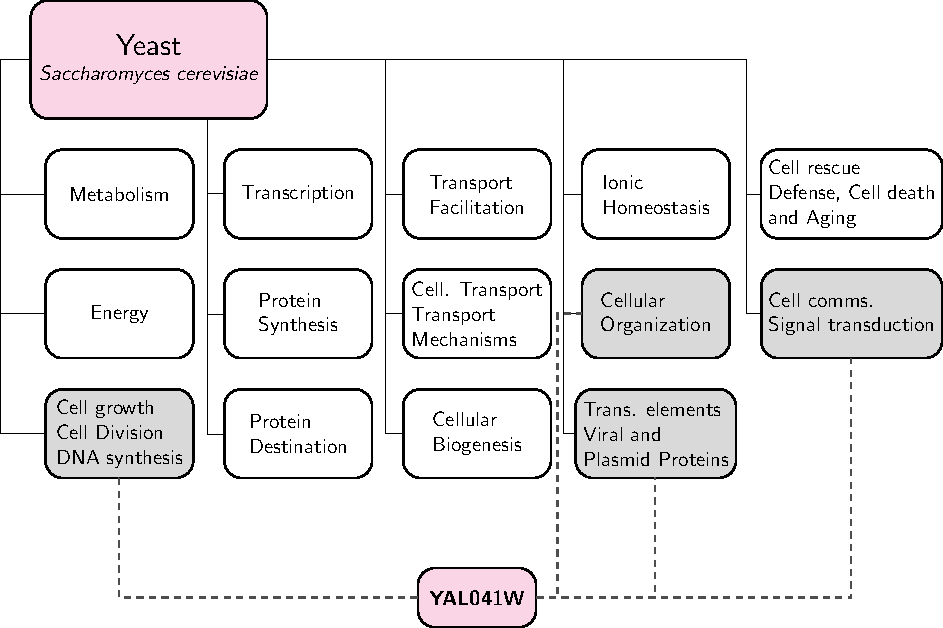
\includegraphics[width=0.65\textwidth]{ch01/demo_ontology}
  \caption{Functional categories of protein YAL041W in \textit{S. cerevisiae}}
  \label{demo:yeast_go}
\end{figure}

\par We define a set of protein functions or \textit{labels} as a binary
matrix $\mathbf{Y}$ where each row $i=1 \dots N$ is a protein sample, and
each column $j=1 \dots q$ is a protein function (designated as $\lambda$).
The size of $q$ depends on the number of possible labels in the dataset. In
addition, a protein labelset (a row vector) $\mathbf{y}_n$ is encoded as a
one-hot vector of size $q$. Say we're given a protein sample $n$ that performs
functions $\lambda_1, \lambda_4,$ and $\lambda_5$ in a set that only has
five functional categories, $q=5$, then we express its labelset as:

\[
    \mathbf{y}_n = \left[\begin{matrix}
        1 & 0 & 0 & 1 & 1
    \end{matrix} \right]
\]

More formally, we represent a set of protein labelsets as $\mathbf{Y} \in
\{0,1\}^{N \times q}$, where each row-vector $\mathbf{y}_n \in \{0,1\}^q$
is a labelset containing $q$ labels $\lambda$. 


\newpage
Together, we have the following definition:

\begin{definition}{}
A protein dataset $\mathcal{D}$ consists of $N$ pairs of feature and label
vectors $\{(\mathbf{x}_i, \mathbf{y}_i)\}_{i=1}^{N}$ where $\mathbf{x}_i \in
\mathbb{R}^d$ and $\mathbf{y}_i \in \{0,1\}^q$. In matrix-form, $\mathcal{D}$
consists of feature and label matrices, $\mathcal{D} = \langle \mathbf{X},
\mathbf{Y} \rangle$ where $\mathbf{X} \in \mathbb{R}^{N \times d}$ and
$\mathbf{Y} \in \{0,1\}^{N \times q}$.
\end{definition}

\par We will use this definition as we formulate the protein function
prediction problem as a multilabel classification task.


\section{Multilabel classification}
\label{MultilabelClassification}

\par In typical classification tasks, two kinds of data are presented:
the \textit{features}, denoted by the matrix $\mathbf{X} =
(\mathbf{x}_{1}, \mathbf{x}_{2}, \dots, \mathbf{x}_{N})$, describing
a measurable characteristic from the system being observed, and the
\textit{labels}, denoted by the matrix $\mathbf{y} = (y_{1}, y_{2}, \dots
y_{N})$, categorizing the features into classes. A sample $i$
can be defined as a joint feature-label pair $(\mathbf{x}_{i}, y_{i})$ and a
dataset $D$ with $N$ samples can then be described as $N$ pairs of feature
and label vectors  $\{(\mathbf{x}_{i}, y_{i})\}_{i=1}^{N}$.

\par Labels are scalar values $y_{i} \in \{0, 1, 2, \dots C\}$ where each digit 
corresponds to a particular class (e.g. for image classification, $0$ is
``person'', $1$ is ``sea'', $2$ is ``boat'' and so on). The goal of
classification is to learn a hypothesis function $h$ such that it minimizes a
cost function $J$. Recall that in this task, only a single class is associated
to a particular sample. Clearly, this does not represent the case of proteins,
given that multiple classes are associated to it. Imagine a picture of a beach:
one can observe not only the ``sea'' nor the ``person,'' but both of them
existing in the same image as shown in Figure \ref{demo:multilabel}.

%\begin{figure}[!t]
%  \centering
%  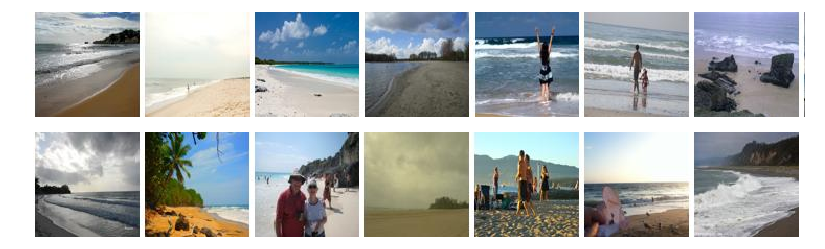
\includegraphics[width=0.70\textwidth]{ch01/demo_multilabel}
%  \caption[Example of multi-label data in image scenes from MIT
%  Places dataset]{
%      Example of multi-label data in image scenes from the MIT
%      Places dataset (\cite{zhou2014learning})}
%  \label{demo:multilabel}
%\end{figure}

\par For multi-label datasets, labels are often defined by vectors instead of
scalars. Here, the notation $\mathbf{Y}$ denotes the whole label matrix
containing $\mathbf{Y} = (\mathbf{y}_{1},\mathbf{y}_{2}, \dots,
\mathbf{y}_{N})$ labelsets for all samples $N$. Each sample $i$ is now defined
by a joint pair of vectors $(\mathbf{x}_{i}, \mathbf{y}_{i})$ rather than a
vector-scalar as seen in a single-label classification task. Thus for each
labelset $\mathbf{y}_{i}$ of size $L$, there exists $\mathbf{y}_{i} =
(\lambda_{1}, \lambda_{2}, \dots, \lambda_{L})_{i}$ where $\lambda_{l} \in \{0,
1\}$. The value $L$ corresponds to the number of possible labels $\lambda_{l}$
in the whole dataset. For a given protein sample, a value of $\lambda_{l}=1$
means that it performs the function $l$, whereas $\lambda_{l}=0$ means
otherwise.

\par There are two main approaches in classifying multi-label data: first by
\textit{problem transformation}, where a multi-label problem is transformed
into separate single-label classification tasks, and the second is
\textit{algorithm adaptation}, where a classifier is designed to 
directly handle multi-label data (\cite{tsoumakas2007multilabel}). This
research will focus on problem transformation, primarily because it is easier
to treat the classifier and the feature extractor as separate modules: the
classifier can be de-coupled from the feature extractor, enabling the former
to be tested on different variants of the latter.  Another reason is that the
literature on problem transformation techniques is extensive enough to
enable benchmark comparisons with different multi-label classifiers in the
future (\cite{zhang2014review, madjarov2012extensive}). The extent
of this work focuses on a specific technique called \textbf{binary relevance},
and will be treated as the baseline during the experiments.

\par Binary relevance (BR) is a problem transformation technique that
decomposes a multi-label problem into a series of single-label classification
tasks (\cite{boutell2004learning, tsoumakas2007multilabel}). This means that a
classifier $h$ is trained on each label $\lambda_l$ of $\mathbf{Y}$, training
a total of $L$ classifiers. Further modifications can be done to binary
relevance such as training a combination of labels, or building chains of
classifiers (\cite{read2009classifier}). However, due to BR's conceptual
simplicity and time-complexity\footnote[2]{
    Most problem-transformation techniques have an overhead time-complexity
    depending on the classifier $h$. For Binary relevance, we have $\bigO(L
    \cdot h(N, M))$. At inference, the complexity is $\bigO(L
    \cdot h'(M))$. This is relatively faster compared to Classifier Chains
    $\bigO(L \cdot h(N, M + L))$ or Label Ranking $\bigO(L^{2} \cdot h(N, M))$
    (\cite{zhang2014review}).
}, it has been widely used
in most literature (\cite{zhang2017binary}).

\par This research will concentrate on finding good representations for the
binary relevance classifier to solve the problem of protein function
prediction. Specifically, a binary relevance Support-Vector Machine (SVM) will
be utilized. This process of obtaining new features from raw data is called 
\textit{feature extraction} and will be one of the core ideas in this work. Even
if a BR classifier can stand on its own, it is hypothesized that higher
performance is achievable when using the extracted features as compared to the
raw data itself.

\section{Feature Extraction}
\label{FeatureExtraction}

\par Feature extraction can be best illustrated with the \texttt{XOR} gate.
Here, we take its two inputs $\mathbf{x}_{i} = (x_{1}$, $x_{2})_{i}$ as features
and its output $y_{i} \in \{0,1\}$ as the label. With $N=4$ samples
representing all possible bit-combinations, a ``dataset''
$D=\{(\mathbf{x}_{i}, y_{i})\}_{i=1}^{4}$ can be constructed as:

\[
    D = \{(0,0,0), (0,1,1), (1,0,1), (1,1,0)\}
\]

Assuming we only have access to a linear classifier, the feature-space shown
in Figure  \ref{demo:xor} (\textit{left}) proves that classifying the samples is
difficult due to its linear inseparability\textemdash that is, drawing a single
line to perfectly separate the \texttt{X}'s and \texttt{O}'s is impossible.
However, if a new feature-space $\mathbf{\widehat{x}}$ is engineered in such a
way that $\mathbf{\widehat{x}} = (\widehat{x}_{1}, \widehat{x}_2)$ where 
$\widehat{x}_{1} = \text{\texttt{AND}}(\bar{x}_{1}, x_{2})$ and $\widehat{x}_{2}
= \text{\texttt{AND}}(x_{1}, \bar{x}_{2})$, then it is possible to transform $D$
into dataset $\widehat{D}=\{(\mathbf{\widehat{x}}_{i}, y_{i})\}_{i=1}^{4}$
where:

\[
    \widehat{D} = \{(0,0,0), (1,0,1), (0,1,1), (0,0,0)\}
\]

\noindent it can be seen from Figure \ref{demo:xor} (\textit{right}) that 
$\widehat{D}$ is a linearly separable problem solvable by any simple classifier.
In this demonstration, it is evident that hand-engineering features, or
\textit{extracting new features} has been helpful. However, with large
datasets, it will be tedious to manually find useful representations from data.
It is much preferred to automate the whole process. Note that  using this
technique is similar to finding a direct encoding from raw inputs to their 
representation. If there is no context of $\mathbf{\widehat{x}}$'s form, then
there's a need to learn a function $f$ such that $f: \mathbf{x} \rightarrow 
\mathbf{\widehat{x}}$.

\begin{figure}[!b]
  \centering
  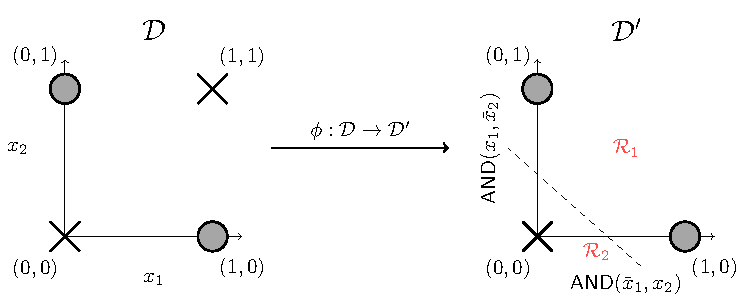
\includegraphics[width=0.70\textwidth]{ch01/demo_xor}
  \caption[Illustration of feature extraction using the \texttt{XOR} gate]{
      Illustration of feature extraction using the \texttt{XOR} gate. Using the
      raw data gives us a linearly inseparable problem \textit{(left)}.
      Constructing new features from raw data transforms the problem into a
      linearly separable one \textit{(right)}
  }
  \label{demo:xor}
\end{figure}

\subsection{The basic autoencoder}


\par This research proposes a feature extraction technique based on the
autoencoder neural network. As a prerequisite, it is necessary to understand
how a basic autoencoder shown in Figure \ref{schema:autoencoder} works.
Here, the function $f$ is obtained by learning a parametric map that directly
encodes the inputs to their representation (\cite{hinton1994autoencoders}).
This method relies on the features $\mathbf{X}$, unlocking correlations and 
relationships that may not be easy to find manually. The literature considers
this kind of technique as \textit{unsupervised learning} 
(\cite{bengio2013representation}).

\par Given a feature set $\mathbf{X}$, the aim is to find a set of parameters
$\theta$ such that the composite function $(g_{\theta'} \circ f_{\theta})
(\mathbf{X})$ minimizes the reconstruction error:

\[
    J(\theta) = L(\mathbf{X}, g_{\theta'}(f_{\theta}(\mathbf{X})))
\]

\noindent Here, the functions $f$ and $g$ are known as the encoder and decoder.
The former encodes the data into a representation $\mathbf{h} = f_{\theta}
(\mathbf{X})$ while the latter attempts to reconstruct $\mathbf{h}$ back into 
$\mathbf{X}$ via $\mathbf{\widetilde{X}} = \mathbf{X} \approx g_{\theta'}
(\mathbf{h})$. Most works implement a tied-weighing scheme (i.e,
$\theta=\theta^{T}$ between the encoder and decoder weights
(\cite{bengio2013representation}). Take note that the
size of $\mathbf{h}$ may not necessarily be the same as $\mathbf{X}$. In sum,
the autoencoder takes an input matrix and faithfully reconstructs it given a
bottleneck (the size of $\mathbf{h}$). This may sound trivial, but due to the
\textit{encoding layer}  $\mathbf{h}$, interesting structure is learned from
the data. The learned representations $\mathbf{h}$ are treated as the new
input $\mathbf{\widehat{X}}$  (similar to the \texttt{XOR} problem) for a
classifier. With a good set-up and optimization scheme, it is even possible to
compress data using this technique (\cite{theis2017lossy}).

\begin{figure}[!t]
  \centering
  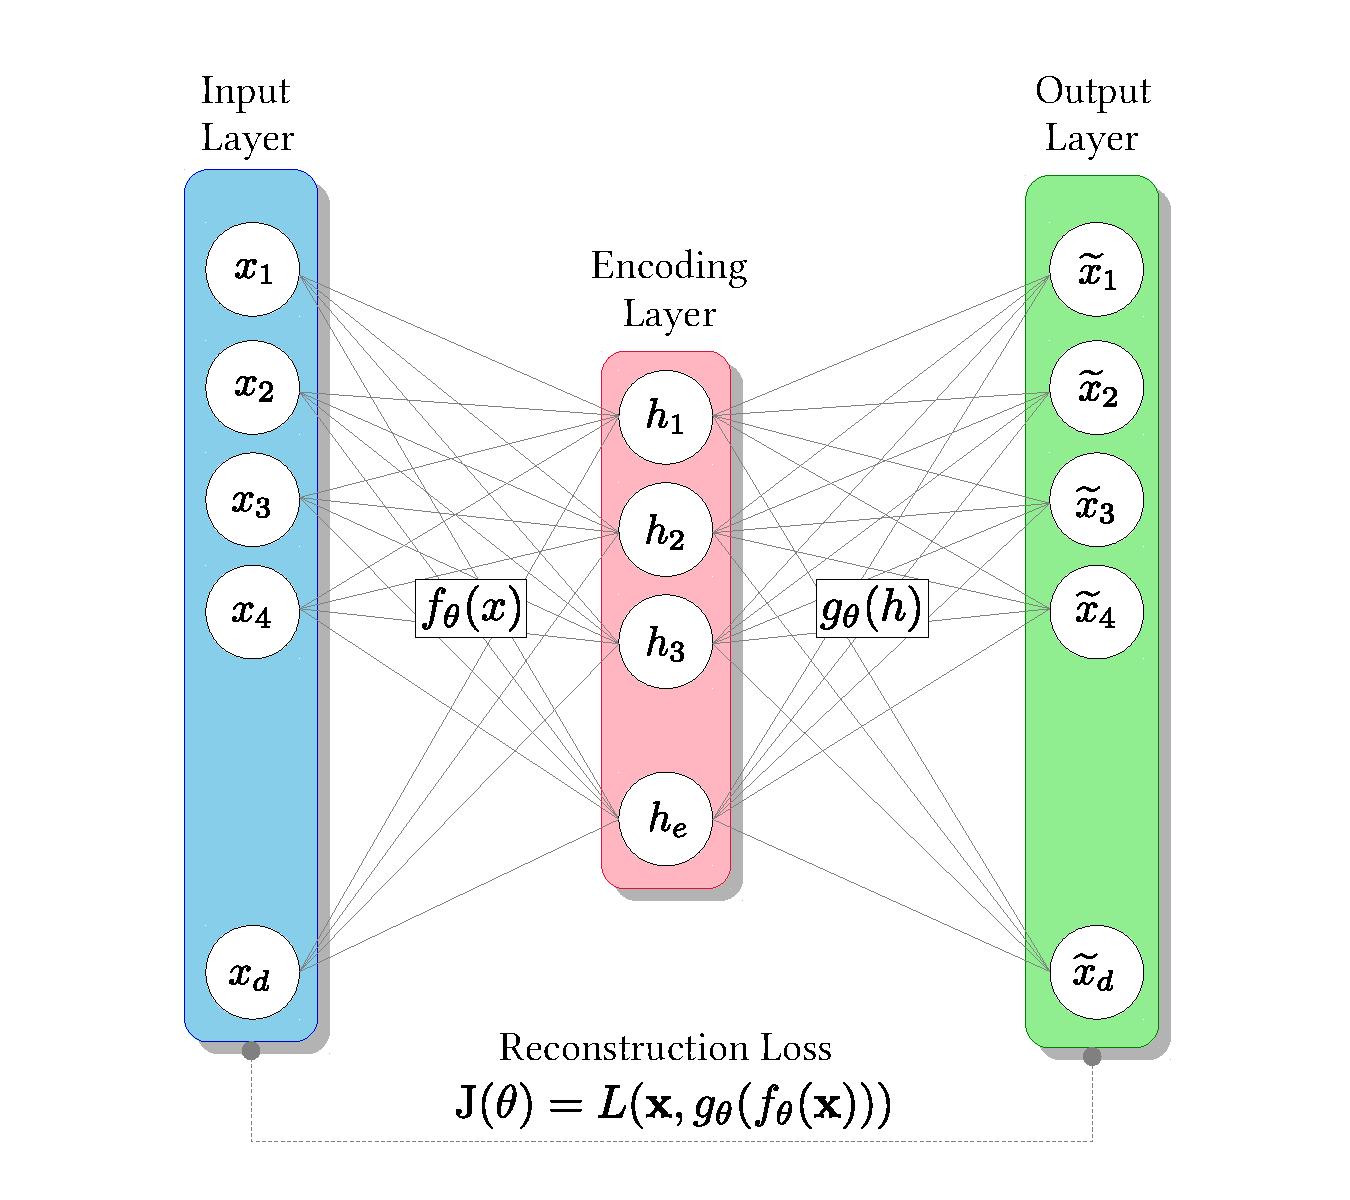
\includegraphics[width=0.60\textwidth]{ch01/schema_autoencoder}
  \caption[Diagram of the basic autoencoder]{
      Diagram of the basic autoencoder
  }
  \label{schema:autoencoder}
\end{figure}

\section{Literature Review}
\label{LiteratureReview}

\section{Motivation}
\label{Motivation}

\par Although extracting features using an autoencoder has been helpful for
classification, one shortcoming of this technique is its tendency to learn
trivial representations from sparse and high-dimensional data
(\cite{wang2017feature, chen2017kate})\textemdash types of data characteristic
of proteins. This is usually the case when the optimization task is to learn
an approximation to the identity $\mathbf{X} \approx \mathbf{\widehat{X}}$,
favoring irrelevant features by overfitting instead of learning a generalized
pattern or representation. Motivating the autoencoder to create relevant features
for the classification task is then important.

\par To address this issue, this work proposes an autoencoder architecture that
extracts a set of sparse yet relevant features. This is done through mutual
competition: the neurons on the network compete based on their activation, and
the ``winners'' absorb the ``losers,'' boosting their importance in the network.
Competition adjusts the backpropagation path, favoring the winners to represent
the input data. This method is task-specific for protein data because only a subset
of its features is considered useful (\cite{iqbal2014efficient, gaudet2017gene}).
The proposed method will be trained on two protein benchmark datasets, and the
extracted features will be used as input to a binary relevance classifier. It will
be compared against a baseline method without feature extraction, and opposed to
existing techniques in literature.

\section{Problem Formulation}
\label{Problem}

\par This research proposes a technique for extracting relevant features from
protein data. It also investigates the effect of feature-relevance to the
performance of a multi-label classifier. Selective feature extraction is
accomplished by encouraging competition between the neurons of an
autoencoder network. In line with this, the following questions will be
answered throughout this work:

\begin{itemize}
    \item How relevant are the learned representations from the proposed method
        as compared to the raw features? (Sec. \ref{FeatureRelevance})
    \item How well does a multi-label classifier perform when using the
        features extracted by the proposed method? (Sec. \ref{ModelQuality})
    \item How well does the proposed method compare with other techniques in
        literature? (Sec. \ref{Benchmarking})
    \item How well do the hyperparameters improve the basic autoencoder and
        affect model performance? (Sec. \ref{AblationTest})
\end{itemize}

